\chapter{基于注意力机制重新表征的缺失值时间序列异常检测}[Complements]

\section{引言}[Introduction]
在数据挖掘中,异常检测指的是对不符合预期模式的项目、事件或观测值的识别。异常检测 已被用于许多重要领域,如视频监控、网络入侵检测、信用欺诈检测、电力行业和医疗保健。

在信息工业快速发展的当代,互联设备和传 感器的数量迎来了快速的增长。这些基于互联设备和传感器所组成的现实系统是现代生活的必要基础。例如日常生活中大量的车联网系统, 电网系统,水处理厂,交通和通信网络等关键的基础设施。这些现实系统涉及大量相互连接的传感器,同时这些传感器每时每刻都在产生大量的观测值。这些通过时刻信息所组织起来的观测值序列称为时间序列,对于一个时刻包含多个观测值的时间序列称为多元时间序列。

这些系统承载了现代人类的生产生活,监控 这些传感器所产生的时间序列,并确保系统免受 攻击的需求越来越高。传统异常检测方式主要依靠数据专家,业务专家等人力进行排查。然而随着现实系统中传感器的数量增多,从这些系统中所收集到的多元时间序列的维度也越来越高,不同指标之间的复杂性也越来越大。使用传统异常检测方式来发现异常变得越来越困难,如何自动化执行多元时间序列的异常检测任务变得越来越重要。

近年来随着数据科学的进步以及人工智能技术的发展,提出了一些基于数据挖掘和深度学习的异常检测方法。Dai 等人采用 RNN 的方法捕捉时间序列沿时间轴变化的趋势,同时引入贝叶斯网络描述不同时间序列之间的关系,最后采用基于标准化流重建的方式进行异常检测,这种方法更侧重于对时间序列沿时间轴方向变化的特征进行建模。Deng 等人采用 GNN 的方法捕捉多个时间序列之间的关联关系,并通过一个全连接层对未来时刻的数据进行预测,以预测值与真实值之间的差异作为异常分数进行异常检测,这种方法更侧重于多元之间序列之间的相关性特征进行建模。Audibert等人基于自动编码器提出了一种基于对抗性学习的重建方法,该方法通过两个自动编码器对抗性学习重建多元时间序列,并以重建值与真实值之间的差异作为异常分数进行异常检测,这种方法更侧重于对数据的整体分布进行建。尽管上述工作都从各自的角度取得了非常好的效果,但他们的工作都是建立在规则,完整且没有任何缺失值的数据集之上。

在真实世界中,往往会因为各种非人为因素 而导致数据采集不全。例如:传输条件的限制,传 感器的自然损坏而没有被及时更换等等。据我们所知,当前并没有算法考虑在缺失值场景下的多元时间序列异常检测。为了验证这些方法在缺失值场景下的真实性能,我们设计了一组实验,如图所示:

实验选取了来自2020年KDD会议中的USAD模型、2021年AAAI会议中的GDN模型、2022年ICLR会议中的GANF模型,这些模型都是多元时间异常检测的SOTA模型。实验包含一个非缺失值场景和两个缺失值场景。实验结果如图1所示,图1中纵坐标是模型的F1性能分数;横坐标 beta = 0、beta = 0.3、 beta = 0.5 指的是实验设计的数据场景。 beta = 0 代表不删除数据, 即模型在其原文中的场景;beta = 0.3 代表删除 30\%的数据,beta = 0.5 代表删除 50\%的数据,即实验设计的缺失值场景。由于直接删除数据无法使模型运行,故我们设定一个原始数据中没有出现过的值作为缺失值的表示填入原始数据当中。 其中每一个点是我们对模型进行了 5 次试验之后所取得的平均值,并且每次试验都会对数据重新随机设置缺失值。
\begin{figure}[ht]
  \centering
  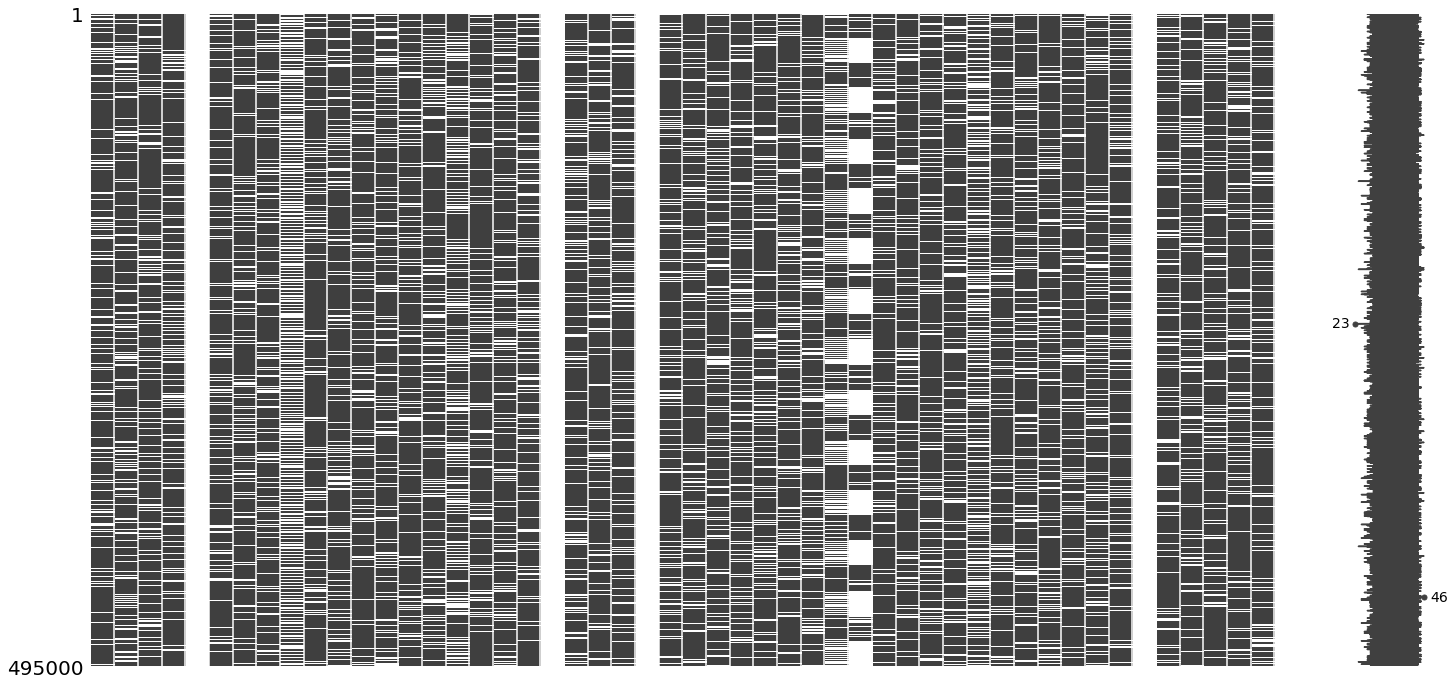
\includegraphics[width = 0.6\textwidth]{chapter3/missing.png}
  \caption{缺失值处理后数据分布情况}
  \end{figure}

试验结果表明模型在存在缺失值的况下都 发生性能的下降,其中 USAD 模型的性能损失最 多,GDN模型的性能下降最少。经过调查发现,USAD 模型是基于数据整体分布建模并重建的方法,缺失值的引入影响了模型对非缺失值数据的建模与重建,致使模型性能下降;GDN 是面向多元时间序列间关联性建模的方法,其更侧重于从数据中学习不同维度的时间序列之间关联性,在一定数据缺失的情况仍然能够鼓励模型学习多元时间序列之间的关联性。但尽管如此,GDN 模型的性能仍然在 beta = 0.3 和 beta = 0.5 的场景下相比原性能下降了 26\% 和 28\%。

\begin{figure}[ht]
    \centering
    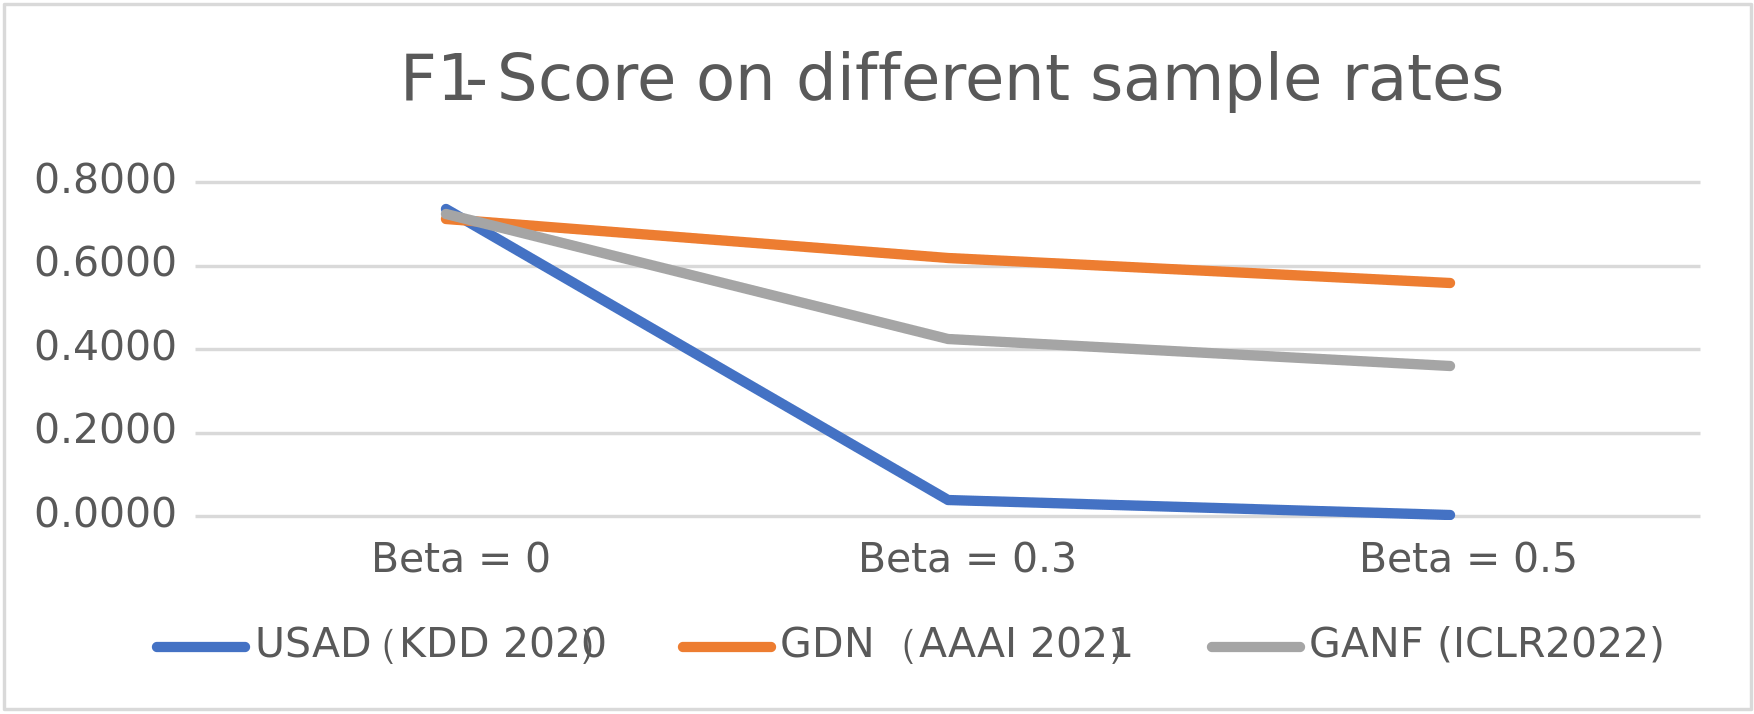
\includegraphics[width = 0.8\textwidth]{chapter3/compare1.png}
    \caption{缺失值场景下SOTA模型性能表现}
    \end{figure}
  
  综上我们可得到结论,传统 SOTA 模型在我 们模拟的缺失值新场景下性能会发生较大下降, 无法满足真实场景下存在缺失值时的性能需求。 如何保证多元时间序列异常检测模型在存在缺失 值的场景下依然能够保证良好的性能具有重要的现实意义。


\section{基于注意力机制重新表征的缺失值时间序列异常检测}[Introduction]
综上,本章预计提出如下贡献点:

提出一种面向缺失值的多元时间序 列的异常检测算法MMAD (Missing Multi Time Series Anomaly Detection),该算法首次提出了一种缺失值场景下的多元时间序列异常检测解决方案。

提出的一种掩码注意力机制模块 (MMAR)将包含缺失值的不完整时间序列数据映射为完整的高维嵌入表征,该表征融合了时间信息、缺失值信息以及观测值信息;同时提出一种基于条件标准化流的标准化分布变换模块(CNF-AD)对该表征进行重建,该模块学习一个可逆变换函数实现一个简单分布(例如高斯分布)与真实分布近似之间的映射,通过该函数与简单分布计算观测值在真实分布中的近似概率,以该概率作为异常分数进行异常检测。

实验结果表明我们的方法在多维时间序 列异常检测任务上有着良好的表现,同时在不规 则时间序列的任务上超越了当前传统异常检测方法。

\begin{figure}[htb]
  \centering
  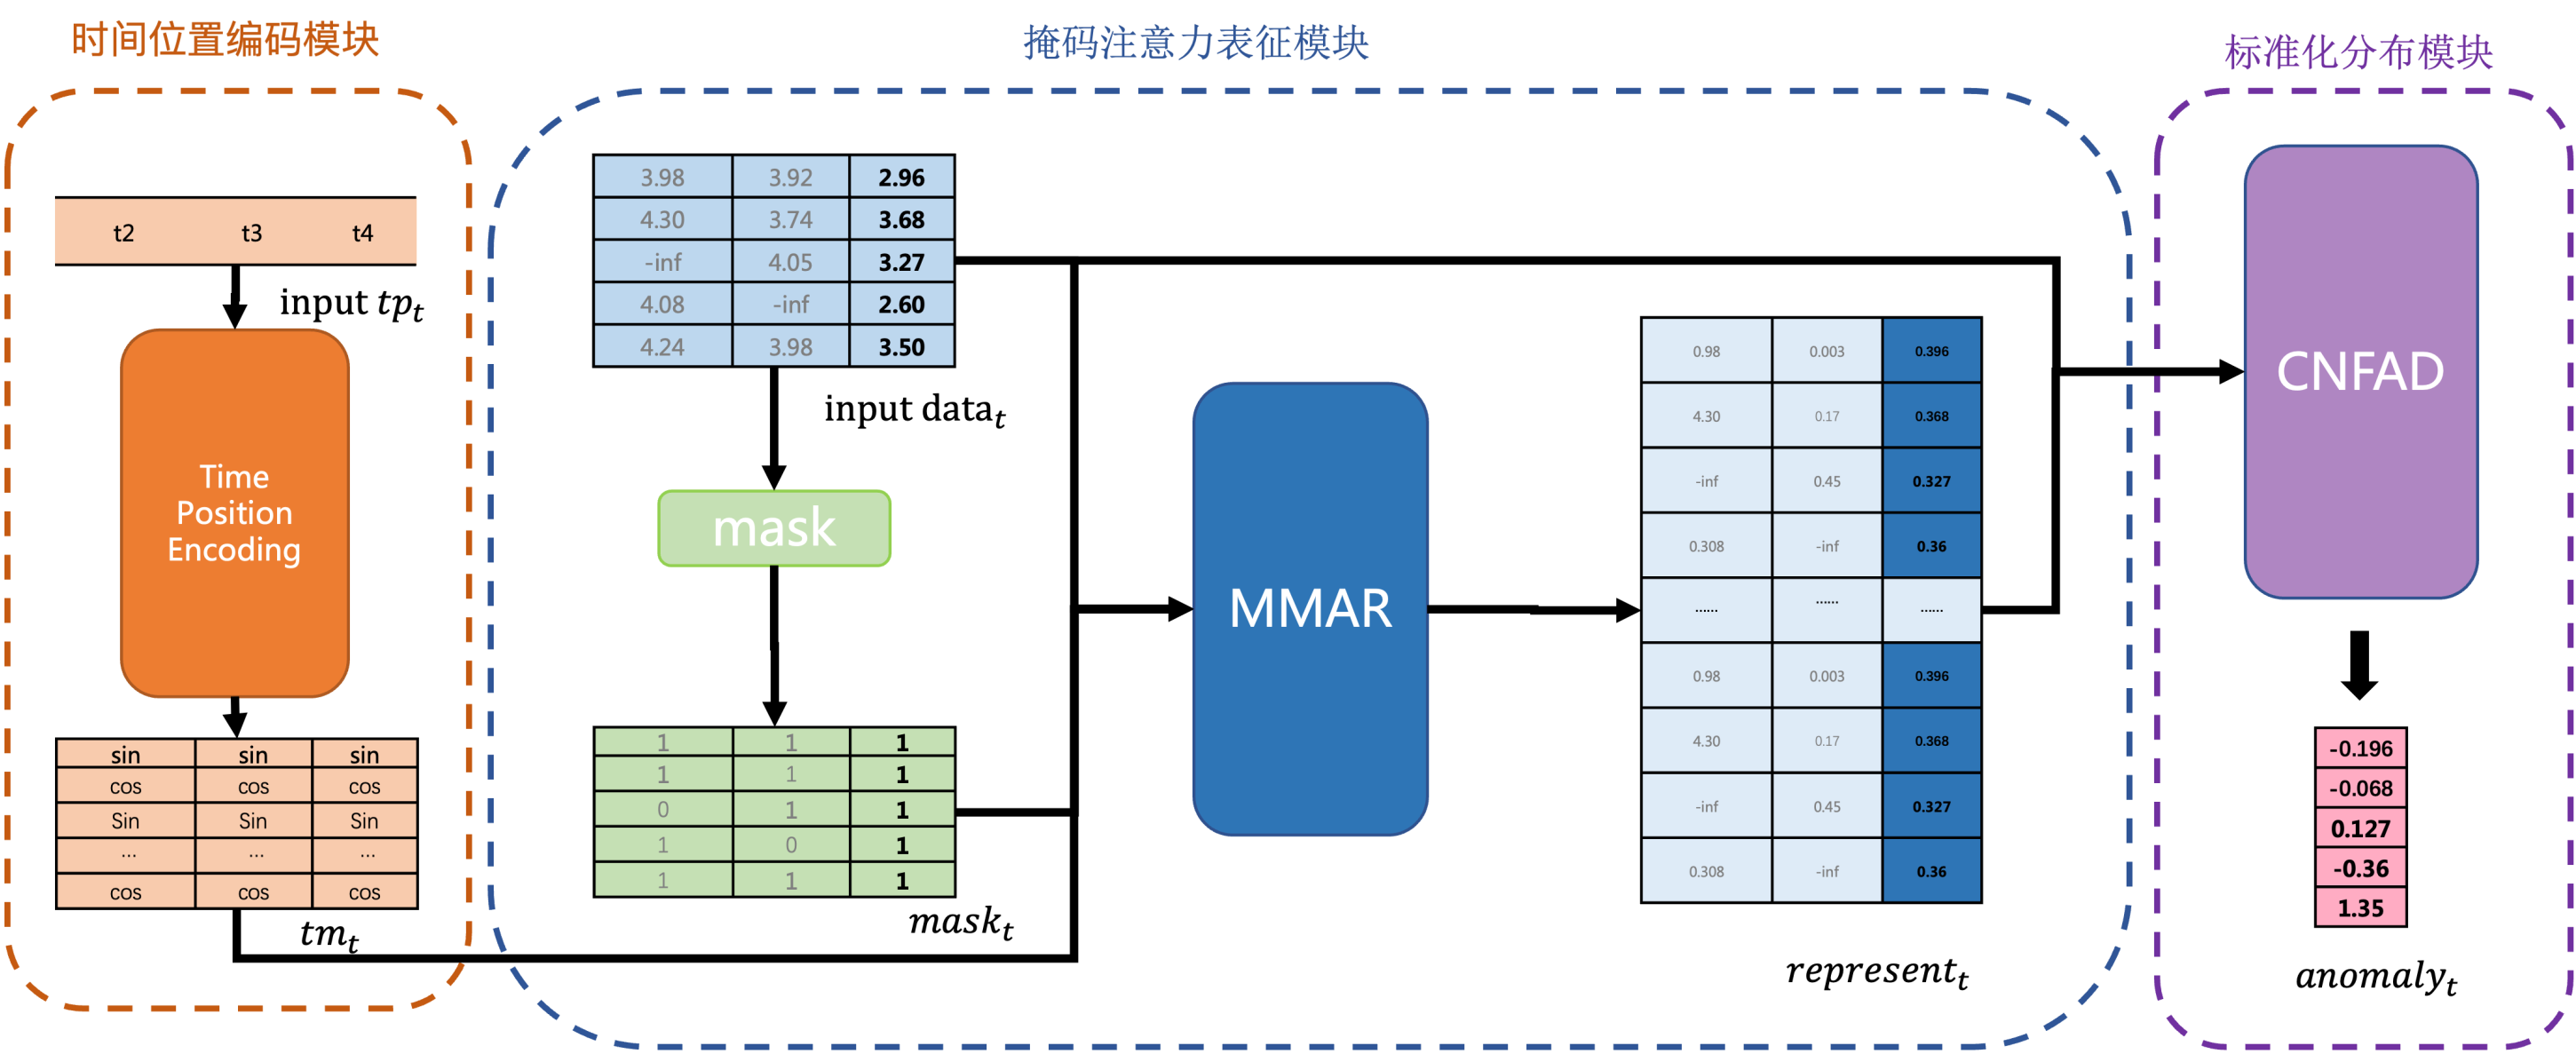
\includegraphics[width = 1\textwidth]{chapter3/overview.png}
  \caption{模型整体架构}
  \end{figure}

模型主要由三个模块组成,即时间位置编码模块(Time Position Encoding)、掩码注意力表征模块(MMAR)和标准化分布变换模块(CNF-AD)。
其中时间位置编码模块的主要目的是将原时间向量$tp_t$ 转换成时间矩阵 $timematrix_t$以建模不同时刻之间的关联关系;掩码注意力表征模块(MMAR) 主要目的是将包含缺失值的不完整时间序列数据映射为完整的高维嵌入表征;标准化分布变 换模块(CNFAD)的目的是学习一个可逆变换函数实现一个简单分布(例如高斯分布)与真实分布近似之间的映射,通过该函数与简单分布计算观测值在真实分布中的近似概率,以该概率作为异常分数进行异常检测。
\subsection{时间位置编码模块}

  时间位置编码模块主要对时间戳进行重新编码,将原来由单个数值的时间戳编码到$d_model$长度的向量以表示更加丰富的信息。对于原来$(t_2,t_3,t_4)$的 $tp_t\in R^{1 x L}$, 所组成的时间戳向量我们会通过位置编码来映射到$timematrix_t$矩阵中。
  \begin{figure}[ht]
    \centering
    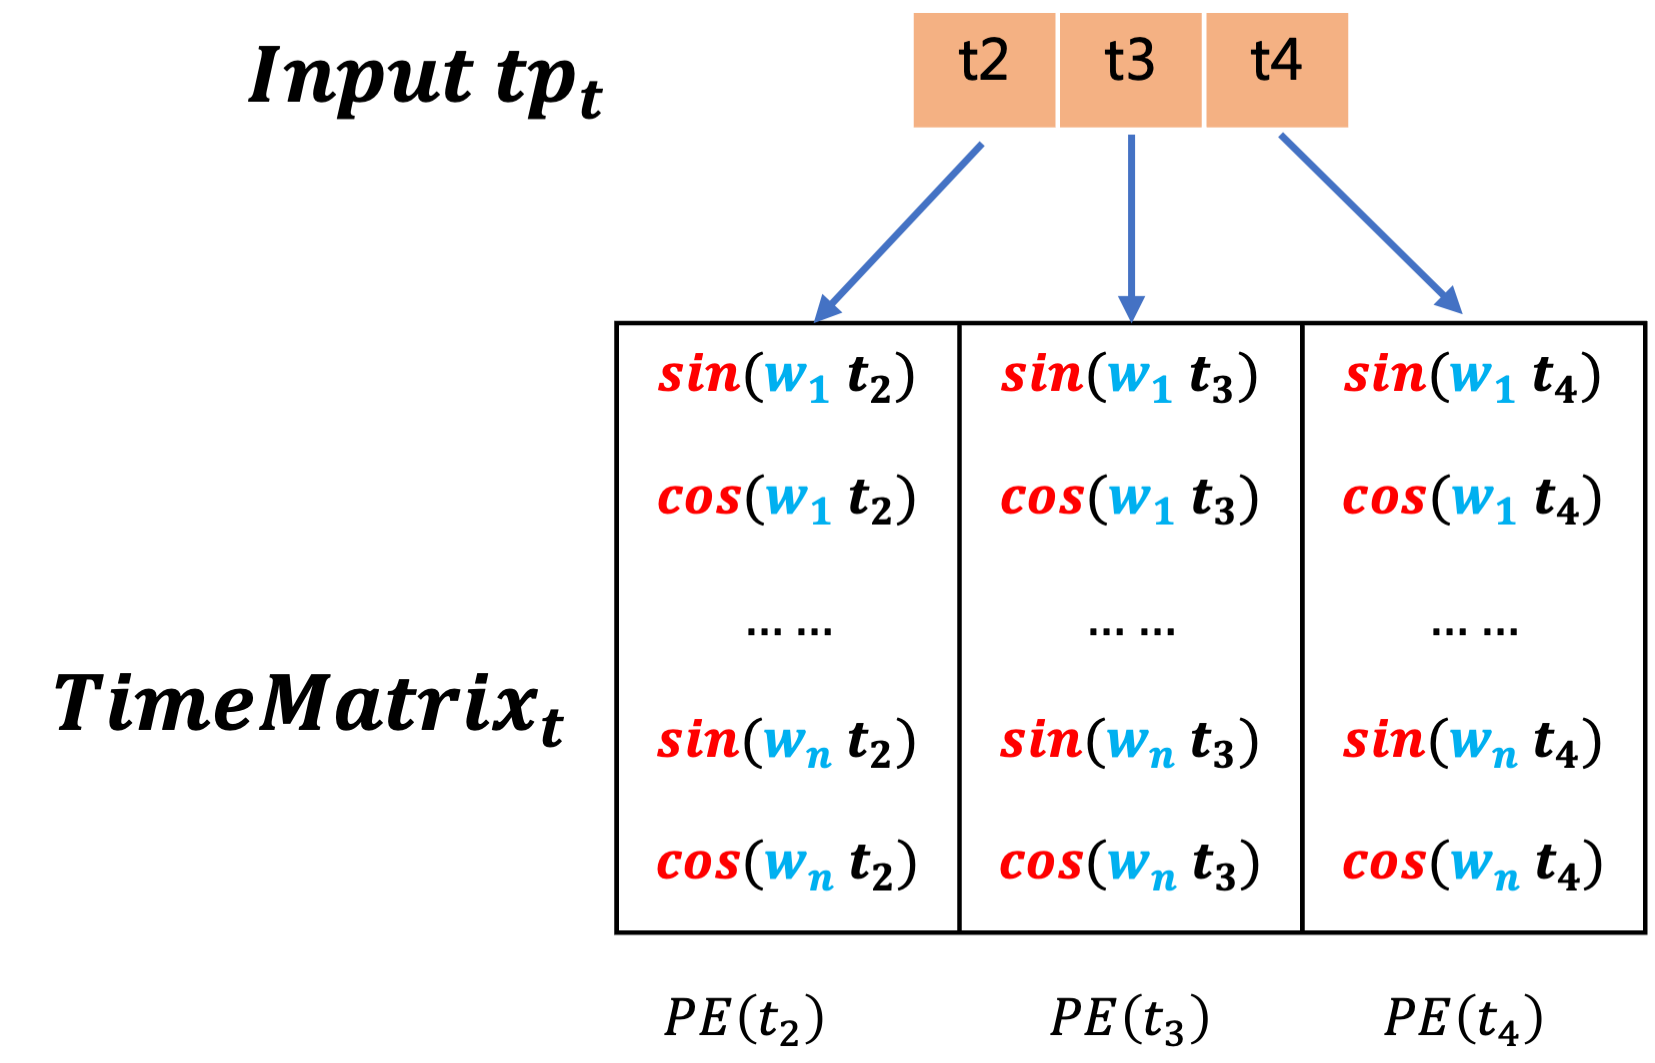
\includegraphics[width = 0.6\textwidth]{chapter3/time1.png}
    \caption{时间向量转化为时间矩阵}
    \end{figure}
  
  
  
  以上图为例子, 原始时间倠是如同“ $2022 / 5 / 13$ 15:03:00” 的格式化日期时间, 首先会将其转化成 UNINX 整数型时间戳 “ 16524380 ” 并作为变量 $t$ 。 通过给时间 $t$ 设置不同的参数 $\frac{1}{1 e 5^{\frac{2 i}{d_{\text {model }}}}}$, 其中 $i$ 为 向量中的标号, $\left(i=0,1, \ldots, \frac{d_{\text {model }}}{2}-1\right) \in(0,1)$ 。
  
  对于不同时刻的同一维度参数相同,我们可 以通过正余弦和公式来推导不同时刻之间的相对 与绝对位置关系:
  \begin{equation}
    \begin{aligned}
    \sin (t+p) &=\sin (t) \cos (p)+\cos (t) \sin (p) \\
    \cos (t+p) &=\cos (t) \cos (p)-\sin (t) \sin (p)
    \end{aligned}
    \end{equation}
  绝对位置关系指的是某时刻 $t$ 与其距离绝对 位置 $p$ 的关系, 由于 $p$ 在此处是一个常数故我 们可以将 $P E(t+p)$ 写成一个关于 $P E(t)$ 和常 数 $P E(p)$ 线性组合:
  \begin{equation}
    P E(t+p)=\alpha P E(t)+\beta P E(p)
    \end{equation}
  对于在后续的注意力机制计算中, 两个不同位置 的关系将通过点积来对其表示, 所以相对位置关 系指的是 $P E(t+p)$ 与 $P E(t)$ 之间的点积。同理 由上面的推导我们也能将 $P E(t+p) P E(t)$ 写成 一个关于 $P E(t)$ 和常数 $P E(p)$ 线性组合:
    \begin{equation}
      P E(t+p) P E(t)=(\alpha P E(t)+\beta P E(p)) P E(t)
    \end{equation}
  
  \begin{figure}[ht]
    \centering
    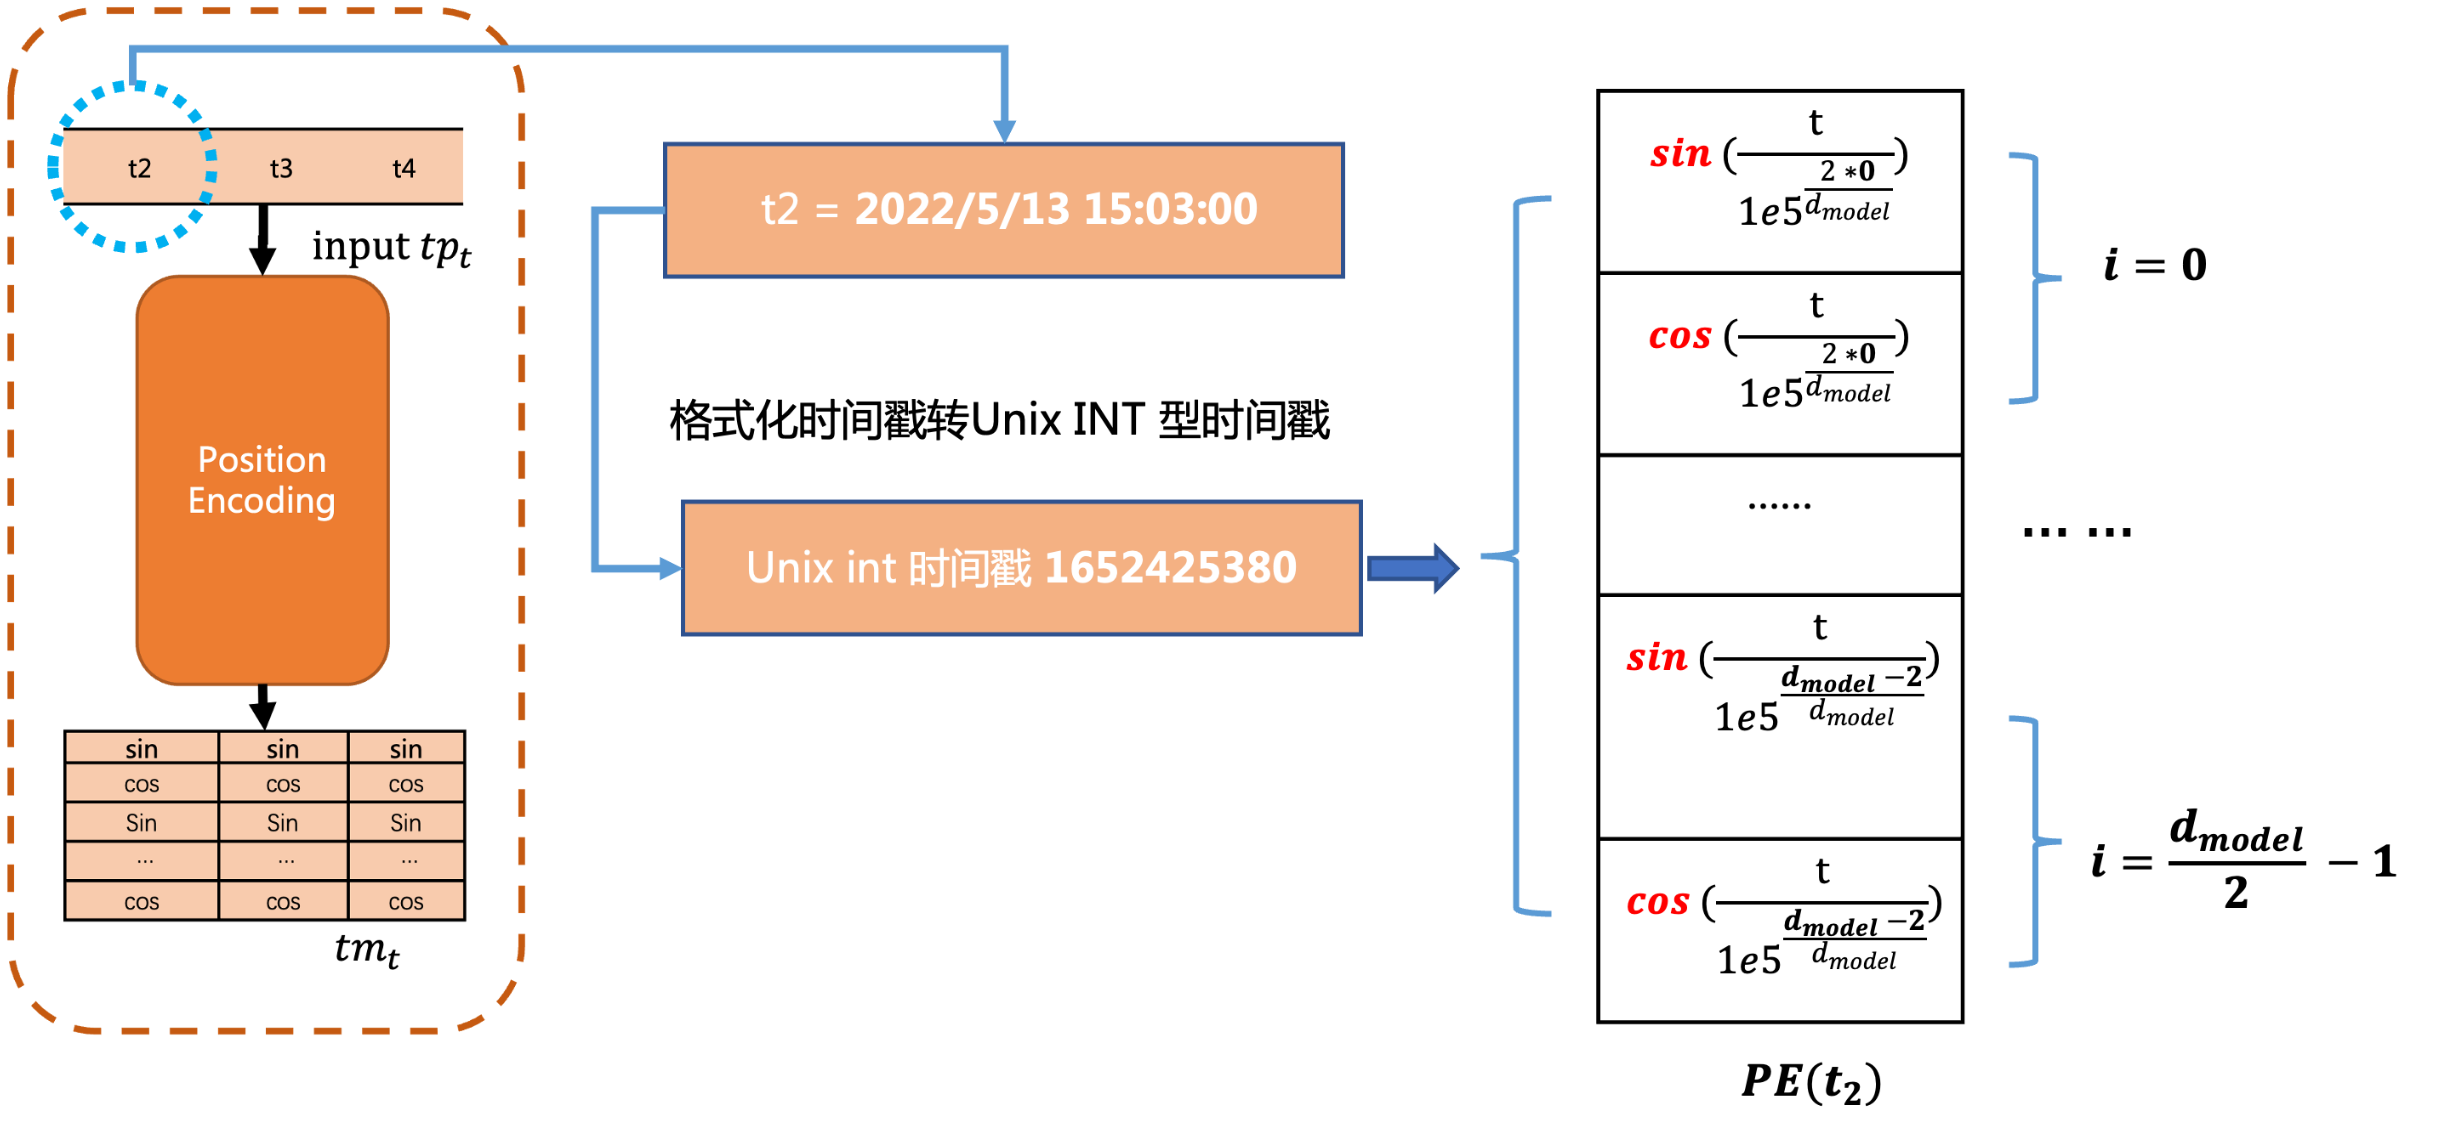
\includegraphics[width = 1\textwidth]{chapter3/time2.png}
    \caption{单个时间戳转换流程}
    \end{figure}
  
  \subsection{掩码注意力表征模块}
  这一模块的主要目的是通过真实数据 $data_t$, 缺失值分布矩阵 $mask_t$, 以及由上一模块所计算 得到的时间矩阵 $timematrix_t$ 来计算得到 的关系,$timematrix $中不同时刻之间的关系, $mask_t$ 中缺失值与非缺失值之间的关系,并用于 后续基于标准化流异常检测的推断。
  
  \begin{figure}[ht]
    \centering
    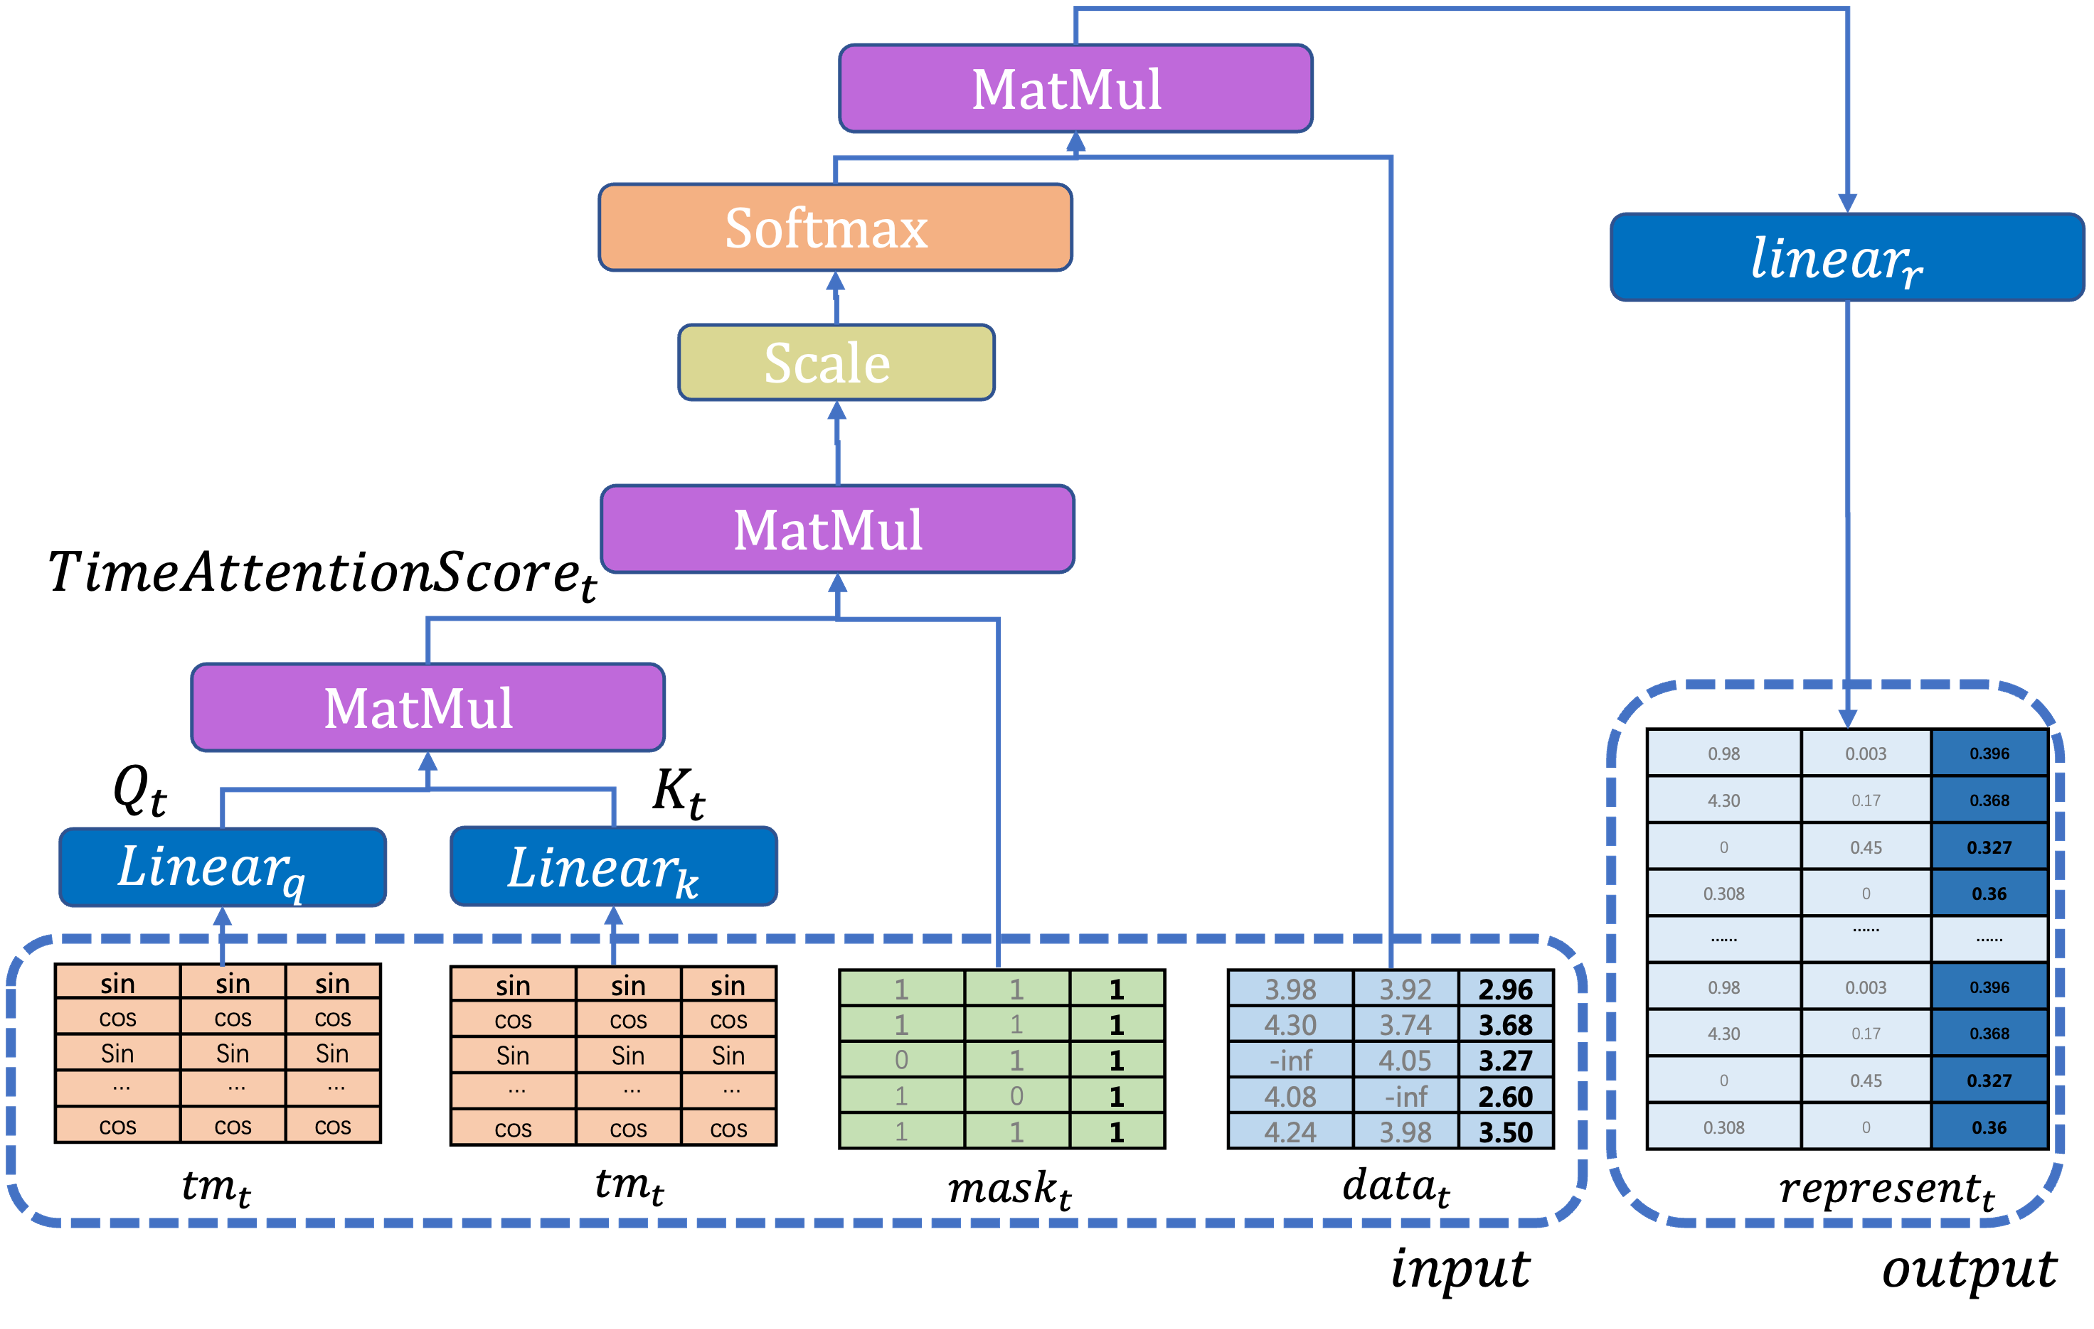
\includegraphics[width = 0.8\textwidth]{chapter3/mask.png}
    \caption{掩码注意力表征模块架构}
    \end{figure}
  
  由上图我们可以看到 MMAR 的细节。MMAR 以$timematrix_t$, $mask_t$, $data_t$ 作为输 入, $represen_t$ 作为输出。
  
  第一步, 通过两个独立线形层$linear_q$,$linear_k$将$timematrix_t$转化为$Q_t, K_t$ 矩阵, 并计根据公式 $\frac{Q_t K_t^T}{\sqrt{d}}$, 计算得到 $TimeAttentionScore_t$, 其中 $d$ 是注意力机制所 到了不同时刻之间的注意力权重。
  
  第二步,融入缺失值信息。首先模型会通过mask模块将$data_t$中的缺失值和非缺失值值进行提取,并用0,1 (0 代表缺失值,1 代表非缺失值)代替得到$mask_t$, 将$mask_t$与刚才与上一步中$TimeAttention_t$ 融合得到最终的面向缺失值注意力分数$maskTimeAttentionScore_t$。
  
  第三步,融入真实数据信息。通过将包含了不同时刻上下文的真实数据 $data_t$ 与包含了不同时刻$maskTimeAttensionScore_t$  进行融合以对$data_t$ 进行重新表征,这一步的目的主要是学习到$data_t $在时间维度上的的主要分布。
  
  第四步,我们利用一个线性层$linear_r$将上一步得到的$maskTimeAttentionData_t$ 映射到高维空间即 
  \begin{equation}
    represent_t=linear_r(maskTimeAttentionData_t)
  \end{equation}
  
  \subsection{标准化分布变换模块}
  \begin{figure}[ht]
    \centering
    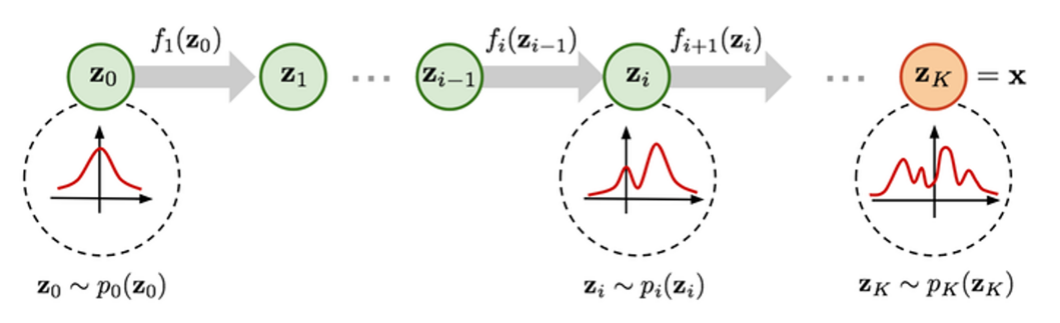
\includegraphics[width = 1\textwidth]{chapter3/nf2.png}
    \caption{标准化流原理解释}
    \end{figure}
  
  在获取到$represent_t$之后,我们需要依据这些信息对观测值进行是否异常的判断。传统异常检测方法往往基于AE, VAE 等生成模型对生 成的编码进行重构,并用生成数据与真实真实数 据的差异作为异常分数,这种方式最大对于生成 模型的输入编码要求很高,需要非常准确的捕捉 到数据的真实分布。
  我们采用了一种基于标准化流的异常检测模 型并加以改进,标准化流并不直接生成真实数据,而是尝试学习一种变换,将类似于正态分布等简 单分布进行一系列的可逆变换以逼近真实的数据分布。
  如图所示
  
  \begin{figure}[ht]
    \centering
    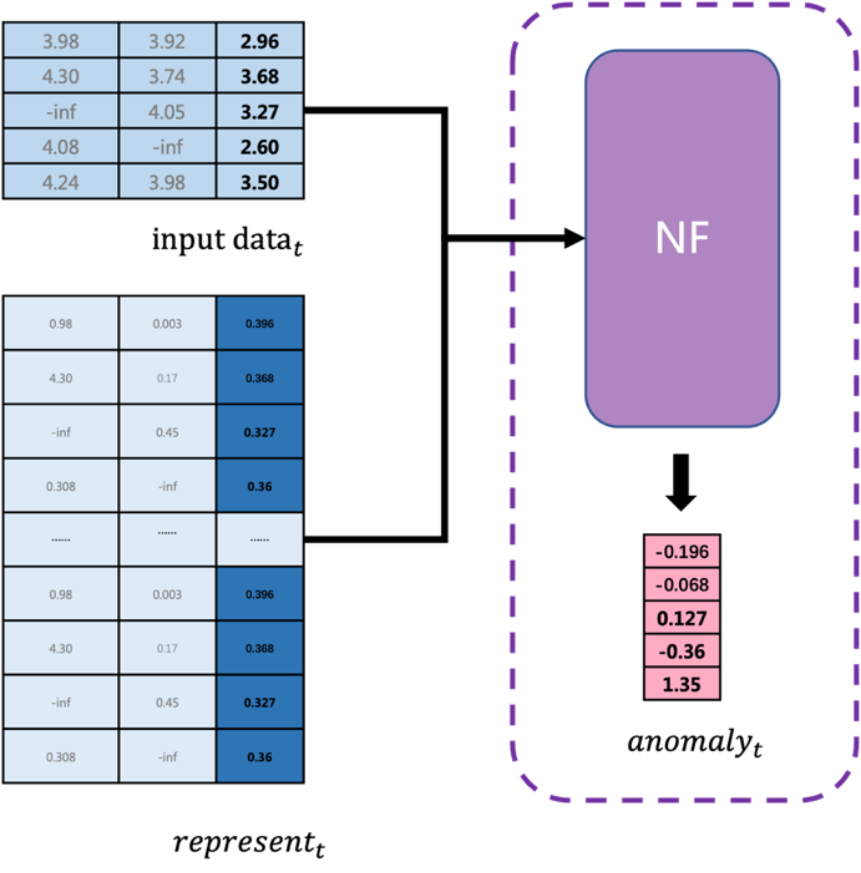
\includegraphics[width = 0.6\textwidth]{chapter3/nf1.png}
    \caption{标准化分布变换模块架构}
    \end{figure}
  
  据概率密度的变换定理,如果$y =f(x) $且 $f$ 是可逆的那么存在:
  \begin{equation}
    \begin{gathered}
    p_x(x)=p_y(f(x)) *|\operatorname{det} J f(x)| \\
    p_y(y)=p_x\left(f^{-1}(y)\right) *\left|\operatorname{det} J f^{-1}(y)\right|
    \end{gathered}
    \end{equation}
  
  如果存在多个可逆 $f$ , 那么在取log 后进行加和
    \begin{equation}
      \begin{gathered}
      z_k=f_k \circ \ldots \circ f_2 \circ f_1\left(z_0\right) \\
      \log _q\left(z_k\right)=\log _{q 0} z_0-\sum_{k=1}^K \log \operatorname{det}\left|\frac{\partial f_k}{\partial z_k}\right|
      \end{gathered}
      \end{equation}
  
  进一步的,我们可以将标准流推广到条件标准化流, 即:
  \begin{equation}
    \log _p(x \mid h)=\log _q(f(x ; h))+\log \left|\operatorname{det} \nabla_x f(x ; h)\right|
    \end{equation}
  
  简单来讲, 在真实分布 $p$ 上取得在满足限制条件 $h$ 的数据 $\mathrm{x}$ 的概率密度 $\log$ 值可以等价于在简单 分布 $q$ 上取得变换后 $f(x ; h)$ 的概率密度 $\log$ 值加上 余项 $\log \left|\operatorname{det} \nabla_x f(x ; h)\right|$ 。
  
  \subsection{训练过程及异常分数设置}
  我们将数据在真实分布上概率密度的log值设为异常分数,令$represent_t$作为当前$data_t$的限制条件,故我们的异常分数设置为:
  
  \begin{equation}
    \begin{aligned}
    &\text { Anomal }_t=\log p\left(\text { data }_t \mid \text { represent }_t\right) \\
    &=\log q\left(f\left(\text { data }_t ; \text { represent }_t\right)\right) \\
    &+\log \mid \operatorname{det} \nabla_{\text {data }_t} f\left(\text { data }_t ; \text { represent }_t\right) \mid
    \end{aligned}
    \end{equation}
  
  其中 $p$ 是真实数据的分布,$q$ 为一种简单分布,例如高斯分布或均匀分布,$f$ 为模型训练得到的可逆变换。
  在多元时间序列异常检测问题中,训练集通常被设置为不存在攻击或异常的时间段所收集的数据;测试集通常被设置为存在攻击或异常的时间段的数据。所以我们的训练目标是使的训练集上的异常分数最小,故我们使用最大似然估计(MLE)作为我们的损失函数:
  
  \begin{equation}
    \begin{aligned}
    &\min G(X) \\
    &=-\sum_{t=1}^{L_{\text {train }}} \log q\left(f\left(\text { data }_t ; \text { represent }_t\right)\right) \\
    &+\log \mid \operatorname{det}_{\text {data }_t} f\left(\text { data }_t ; \text { represent }_t\right) \mid
    \end{aligned}
    \end{equation}

\section{实验结果及分析}[Introduction]
\subsection{实验数据集}
\textbf{SWAT数据集}\cite{swat}: SWaT数据源于与新加坡公用事业委员会协调的运行水处理试验台。该数据以1秒的频率收集持续11天的51个传感器记录。该数据集分为测试集和训练集,其中前7天为训练集,不包含异常或攻击行为,后4天为测试集合,总共进行了36次攻击,其中大约11\%的时间步为异常标签。

\textbf{WADI数据集}: WADI是一个由大量供水管道组成的供水系统。因此,WADI形成了一个更加完整和现实的水处理,存储和分配网络。数据集包含14天正常运行数据,这些数据组成了训练集、在接下来的几天,以不同的时间间隔进行了许多受控的物理攻击,这与测试集中的异常情况对应。

\textbf{SMD数据集}: SMD是从一家大型互联网公司收集的服务器机器数据集,数据集被分为两个等长的部分,其中前半部分为没有发生异常的数据集,可以被用来作为训练集;后半部分包含攻击行为,可以被用来作为测试集。

\subsection{实验设置}

真实世界中往往会因为传输条件的限制,传感器的自然损坏而没有被及时更换等情况而导致数据的缺失,为了模拟真实的数据缺失情况,我们在每个传感器的时间维度上进行均匀采样,并删除采样时间戳上的数据。

在介绍评价指标之前,需要先介绍混淆矩阵。在机器学习领域,混淆矩阵(Confusion Matrix),又称为可能性矩阵或错误矩阵。混淆矩阵是可视化工具,特别用于监督学习,在无监督学习一般叫做匹配矩阵。主要用于比较分类结果和实际测得值,可以把分类结果的精度显示在一个混淆矩阵里面。
混淆矩阵的每一列代表了预测类别,每一列的总数表示预测为该类别的数据的数目;每一行代表了数据的真实归属类别,每一行的数据总数表示该类别的数据实例的数目;每一列中的数值表示真实数据被预测为该类的数目。
其中主要包含四个参数:True Positive(TP):真正类。样本的真实类别是正类,并且模型识别的结果也是正类。False Negative(FN):假负类。样本的真实类别是正类,但是模型将其识别为负类。 False Positive(FP):假正类。样本的真实类别是负类,但是模型将其识别为正类。True Negative(TN):真负类。样本的真实类别是负类,并且模型将其识别为负类。

\begin{figure}[ht]
  \centering
  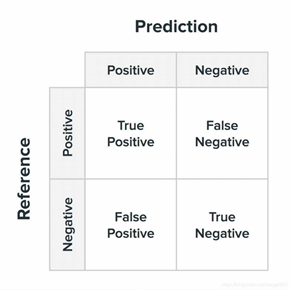
\includegraphics[width = 0.4\textwidth]{chapter4/confusematrix.png}
  \caption{混淆矩阵}
  \end{figure}

多元时间序列异常检测模型一般采用Precision,Recall,F1-Score 作为性能评价指标。其中Precision是检测出某类特征的数量与检测出的所有特征数量之间的比率,衡量的是模型的查准率;一般来说,Precision就是检索出来的条目有多少是准确的。Recall是指检测出的某类特征的数量和数据集中所有的该类特征数量的比率,衡量的是检索系统的查全率。

公式(4-1),公式(4-2),公式(4-3)分别列出了精确度Precision,召回率Recall,F1-Score 的计算方式
\begin{equation}
  \text { Precession }=\frac{T P}{T P+F P}
  \end{equation}

\begin{equation}
  \text { Recall }=\frac{T P}{T P+F N}
  \end{equation}

  \begin{equation}
  F 1=\frac{2 * \text { Precision } * \text { Recall }}{\text { Precision }+\text { Recall }}
  \end{equation}

\subsection{基线模型说明}
\textbf{USAD(Audibert 等,KDD 2020)}采用的是无监督异常检测,在两阶段训练方案下训练两个自动编码器,包括一个共享编码器和两个单独的解码器:自动编码器训练阶段和对抗训练阶段。

\textbf{GDN(Deng 等,AAAI  2021)}采用的是无监督异常检测,将结构学习方法与图形神经网络相结合,着重建模不同维度时间序列之间的关系,另外使用注意力权重来解释检测到的异常。

\textbf{GANF(DAI 等,ICLR  2022)}采用的是无监督异常检测。通过贝叶斯网络建模因果关系的有向无环图(DAG), 通过RNN建模时间序列;引入条件概率作为检测异常分数。

\subsection{总体性能对比}
如表4-1, 表4-2, 表4-3所示,我们测试了不同程度下删除数据后模型性能表现。通过实验结果我们可以看到,我们在SOTA模型的原场景下接近SOTA的性能,
同时在我们设计的新的场景下超过SOTA模型的表现,以此可以证明我们的模型在缺失值场景下具有较好的性能表现。
同时我们的模型在beta = 0 至 beta = 0.3 与 beta = 0.3 至 beta = 0.5 的场景变换中,性能下降最低,这证明了我们的模型在数据损失的情况下性能
下降最不明显,对数据缺失具有鲁棒性。

\begin{table}[htb]
  \caption{所有方法在SWAT数据集上的性能比较}
  %\label{comparison_results}
  \small
  \centering
  \setlength{\tabcolsep}{0.8mm}{
  \begin{tabular}{lccccccccc}\toprule
  Method & \multicolumn{3}{c}{SWAT FULL DATA} & \multicolumn{3}{c}{SWAT DROP 0.3 DATA} & \multicolumn{3}{c}{SWAT DROP 0.5 DATA} \\ \cmidrule(r){2-4} \cmidrule(r){5-7} \cmidrule(r){8-10}
      & F1-Score & Precision & Recall & F1-Score & Precision & Recall & F1-Score & Precision & Recall\\ \midrule
  USAD & 0.7917 & 0.9851 & 0.6618  & 0.5635 & 0.4238 & 0.8408  & 0.3636 & 0.2456 & 0.7003 \\
  GDN & 0.8100 & 0.9935 & 0.6812  & 0.6609 & 0.8167 & 0.5550  & 0.5666 & 0.7271 &  0.4641 \\
  GANF & 0.8065 & 0.9892 & 0.6808  & 0.3048 & 0.2025 & 0.6154  & 0.1314 & 0.0703 &  1.0000 \\
  MMTSAD & 0.7522 & 0.9583 & 0.6191  & 0.6886 & 0.8106 & 0.5986  & 0.6869 & 0.784  & 0.6112 \\
%\bfseries MUSE-Net& \bfseries 2.89 & \bfseries 1.10 & \bfseries 2.74 & \bfseries 1.05 & \bfseries 15.47 & \bfseries 5.47 & \bfseries 14.45 & \bfseries 5.54 & \bfseries 17.19 \\
\bottomrule
\centering
\end{tabular}}
\end{table}


\begin{table}[htb]
  \caption{所有方法在WADI数据集上的性能比较}
  %\label{comparison_results}
  \small
  \centering
  \setlength{\tabcolsep}{0.8mm}{
  \begin{tabular}{lccccccccc}\toprule
  Method & \multicolumn{3}{c}{WADI FULL DATA} & \multicolumn{3}{c}{WADI DROP 0.3 DATA} & \multicolumn{3}{c}{WADI DROP 0.5 DATA} \\ \cmidrule(r){2-4} \cmidrule(r){5-7} \cmidrule(r){8-10}
      & F1-Score & Precision & Recall & F1-Score & Precision & Recall & F1-Score & Precision & Recall\\ \midrule
  USAD & 0.2328 & 0.9947 & 0.1318 & 0.2137 & 0.2551 & 0.1838  & 0.1866 & 0.1897 & 0.1836 \\
  GDN & 0.5700 & 0.9750 & 0.4019  & 0.1389 & 0.0802 & 0.5177  & 0.1092 & 0.1092 & 1.0000 \\
  GANF & 0.3348 & 0.2040 & 0.9324  & 0.2234 & 0.1396 & 0.5584  & 0.1739 & 0.1667 & 0.1818 \\ 
  MMTSAD & 0.3897 & 0.2718 & 0.6883  & 0.2821 & 0.2102 & 0.4286  & 0.2179 & 0.2179 & 0.5844 \\ 
%\bfseries MUSE-Net& \bfseries 2.89 & \bfseries 1.10 & \bfseries 2.74 & \bfseries 1.05 & \bfseries 15.47 & \bfseries 5.47 & \bfseries 14.45 & \bfseries 5.54 & \bfseries 17.19 \\
\bottomrule
\centering
\end{tabular}}
\end{table}

\begin{table}[htb]
  \caption{所有方法在SMD数据集上的性能比较}
  %\label{comparison_results}
  \small
  \centering
  \setlength{\tabcolsep}{0.8mm}{
  \begin{tabular}{lccccccccc}\toprule
  Method & \multicolumn{3}{c}{SMD FULL DATA} & \multicolumn{3}{c}{SMD DROP 0.3 DATA} & \multicolumn{3}{c}{SMD DROP 0.5 DATA} \\ \cmidrule(r){2-4} \cmidrule(r){5-7} \cmidrule(r){8-10}
      & F1-Score & Precision & Recall & F1-Score & Precision & Recall & F1-Score & Precision & Recall\\ \midrule
      USAD & 0.9382 & 0.9314 & 0.9617  & 0.6129 & 0.4713 & 0.8762  & 0.5818 & 0.4392 & 0.8617 \\
      GDN & 0.7183 & 0.7079 & 0.7294  & 0.6263 & 0.5955 & 0.6607  & 0.3517 & 0.2364 & 0.6871 \\ 
      GANF & 0.6241 & 0.5131 & 0.7963  & 0.5983 & 0.4779 & 0.8000  & 0.5808 & 0.4247 & 0.9185 \\ 
      MMTSAD & 0.7949 & 0.9051 & 0.7086  & 0.7025 & 0.7367 & 0.6714  & 0.6491 & 0.5881 & 0.7243 \\
%\bfseries MUSE-Net& \bfseries 2.89 & \bfseries 1.10 & \bfseries 2.74 & \bfseries 1.05 & \bfseries 15.47 & \bfseries 5.47 & \bfseries 14.45 & \bfseries 5.54 & \bfseries 17.19 \\
\bottomrule
\centering
\end{tabular}}
\end{table}

\begin{figure}[htb]
  \centering
  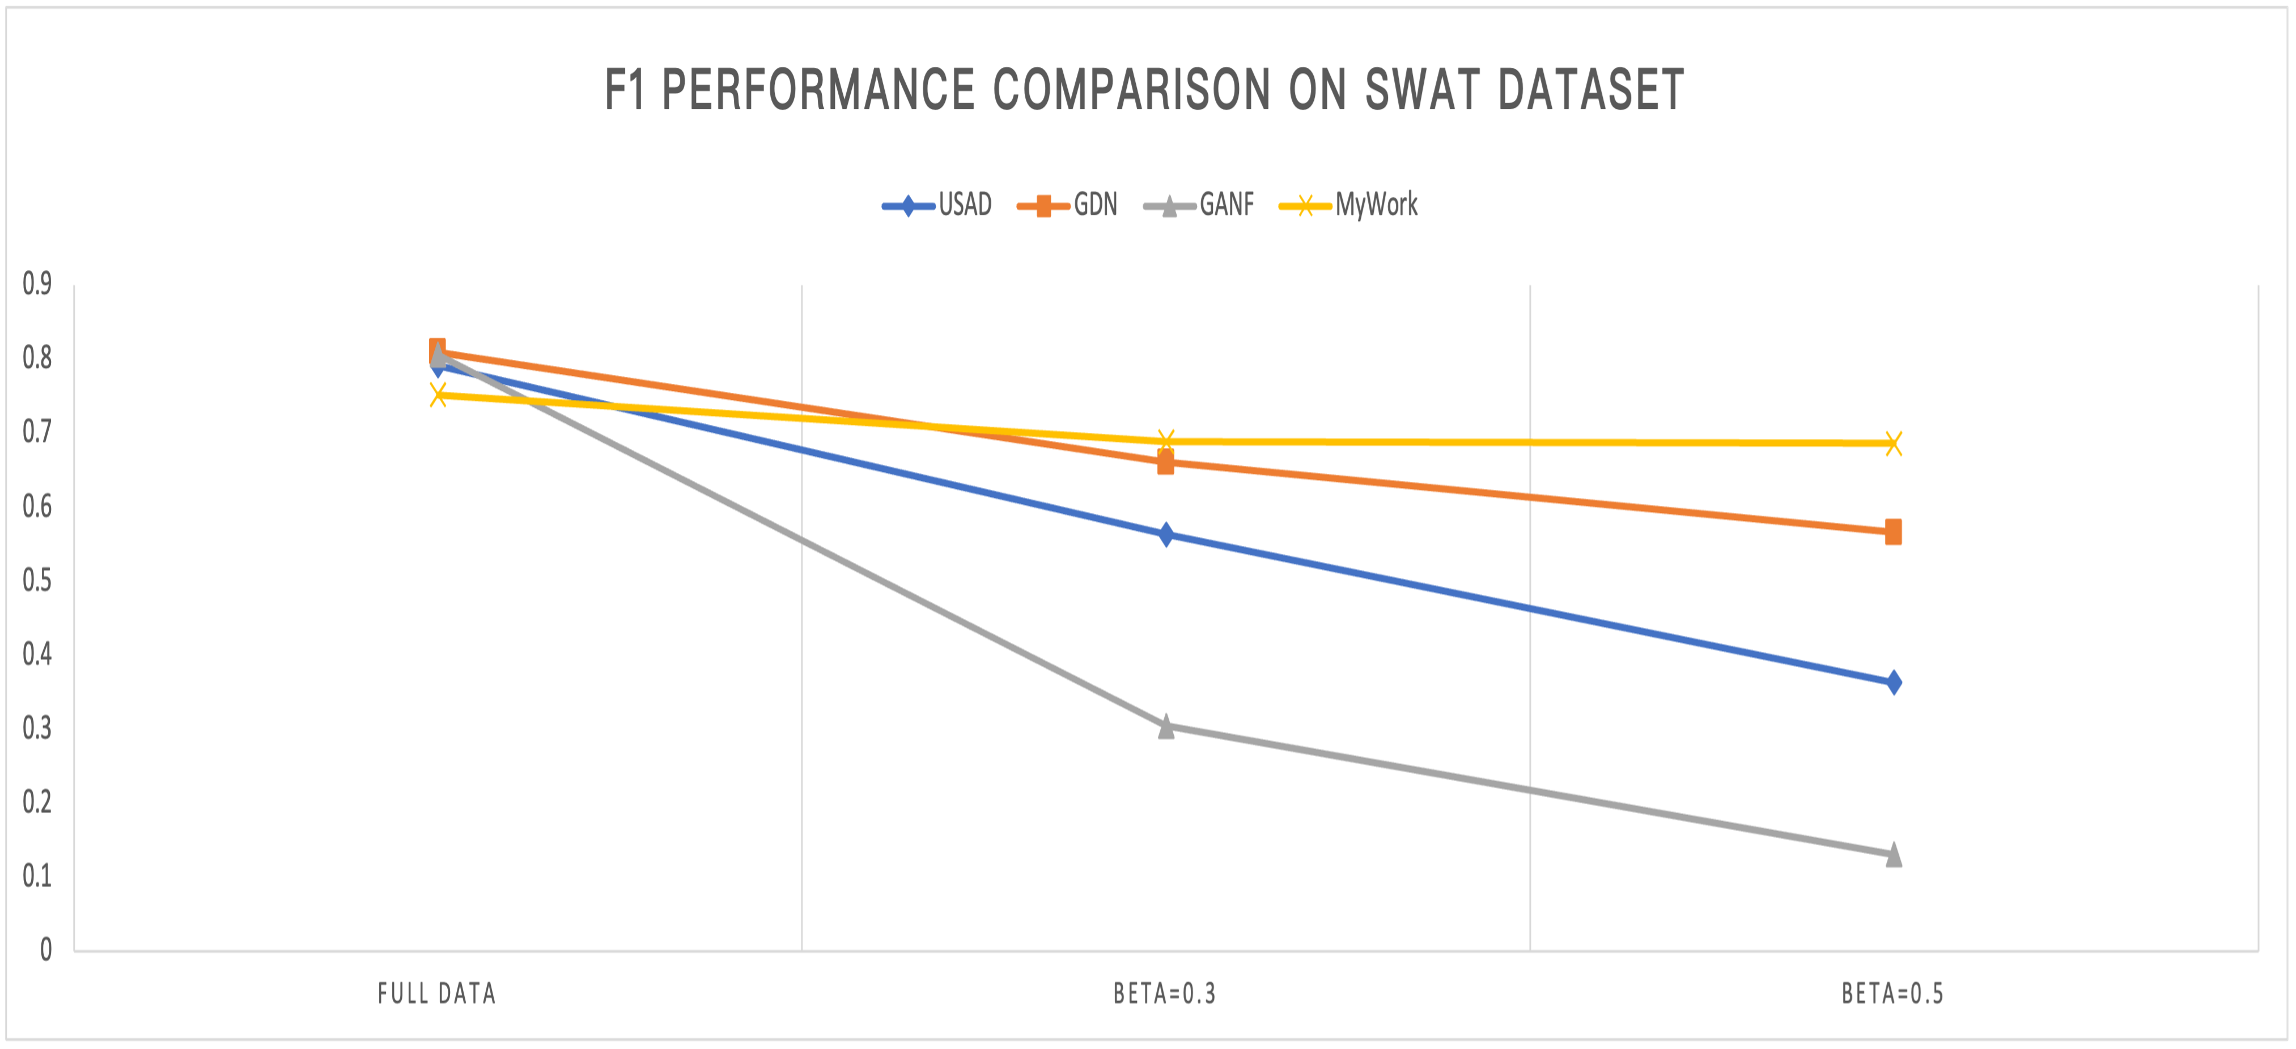
\includegraphics[width = 0.8\textwidth]{chapter4/swat-compare.png}
  \caption{所有方法在SWAT数据集上的性能比较}
  \end{figure}

图4-1展示了SWaT 数据集中对比结果,其中横坐标代表缺失值场景,纵坐标代表F1综合性能分数。可以看到我们在完整数据集下的性能接近当前的SOTA方案,在30\%缺失值的情况下
对比SOTA方案提升约为120\%至4\%,在在50\%缺失值的情况下对比SOTA方案提升约为522\%至20\%。

\begin{figure}[htb]
  \centering
  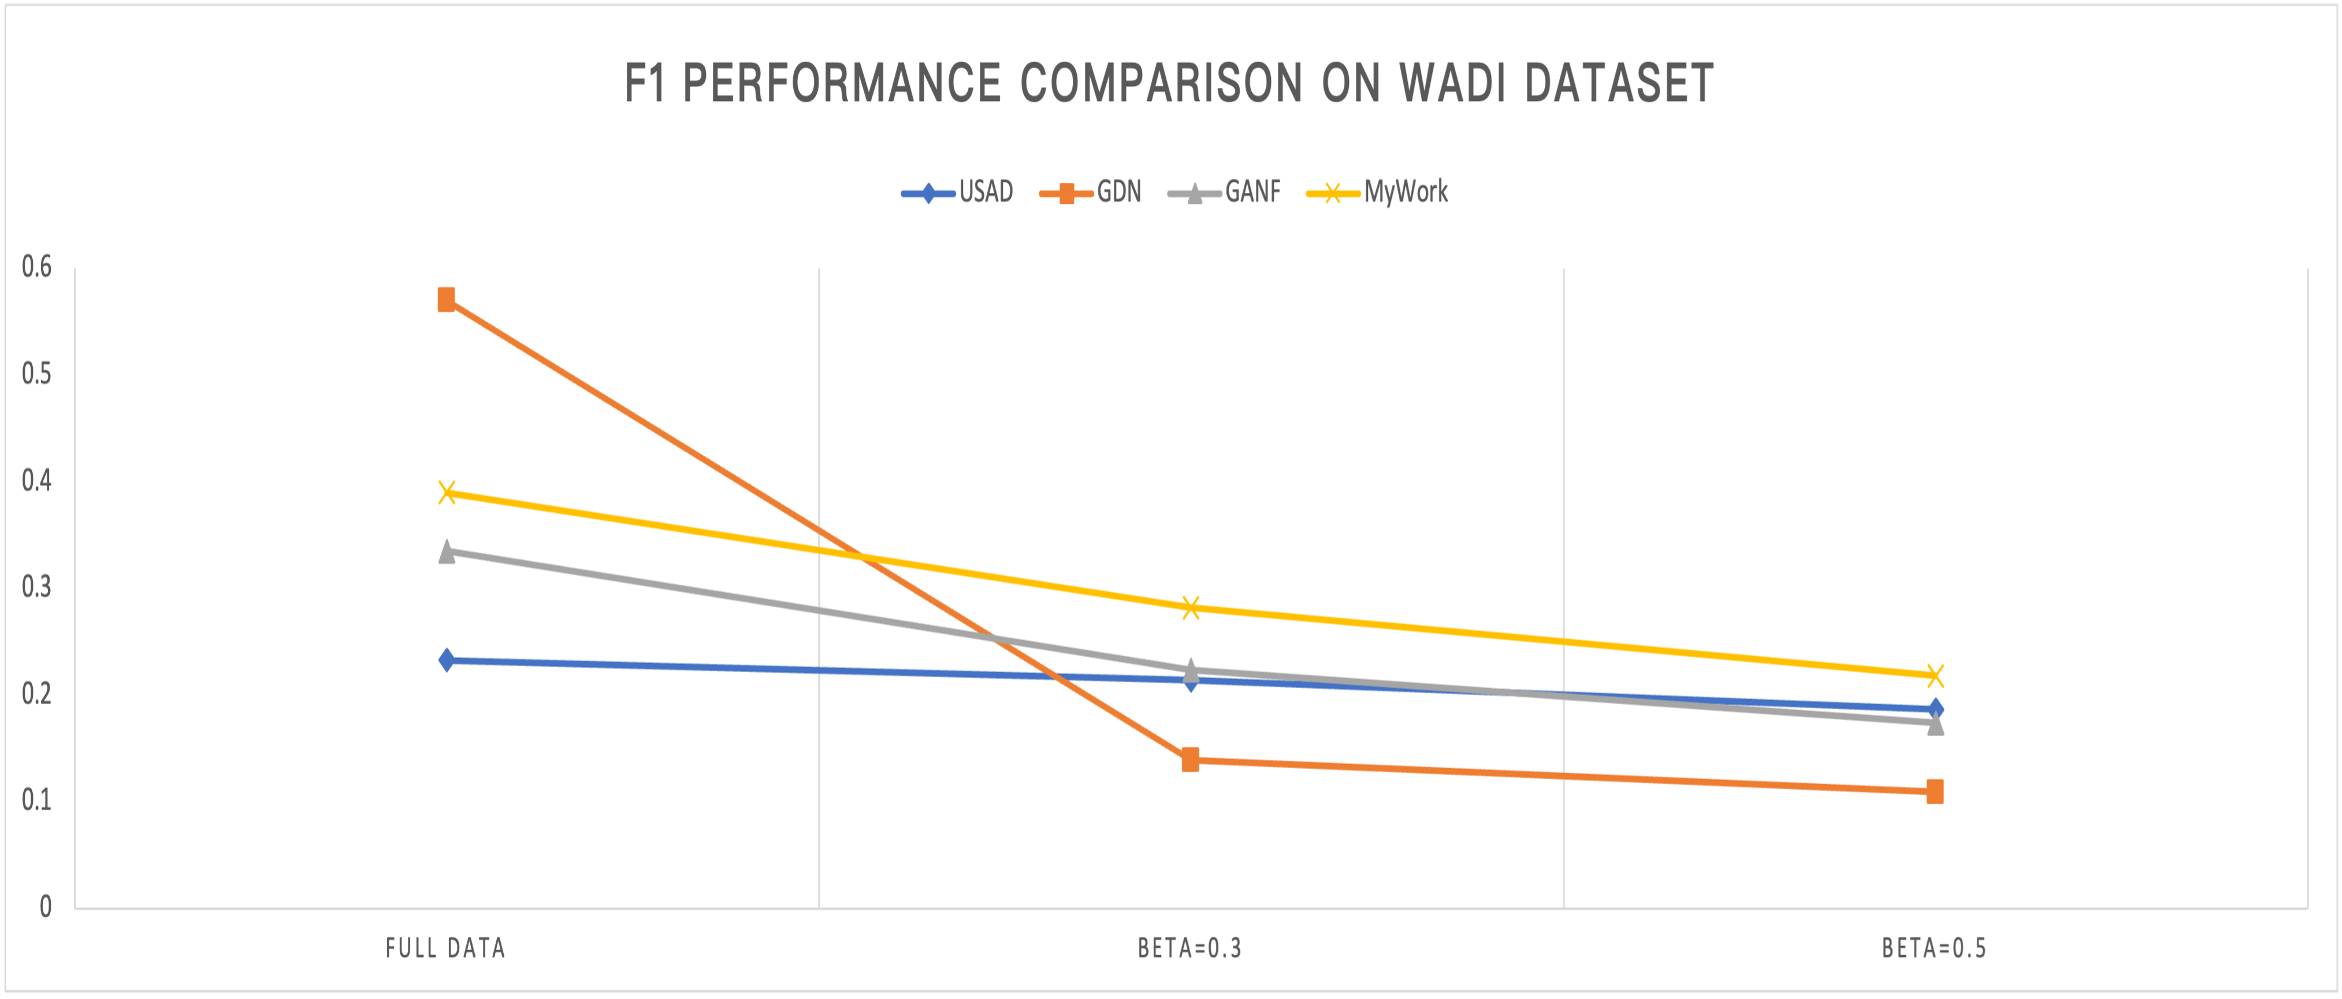
\includegraphics[width = 0.8\textwidth]{chapter4/wadi-compare.png}
  \caption{所有方法在WADI数据集上的性能比较}
  \end{figure}

图4-2展示了WADI 数据集中对比结果,其中横坐标代表缺失值场景,纵坐标代表F1综合性能分数。可以看到我们在完整数据集下的性能接近当前的SOTA方案,在30\%缺失值的情况下
对比SOTA方案提升约为103\%至26\%,在在50\%缺失值的情况下对比SOTA方案提升约为99\%至25\%。

\begin{figure}[htb]
  \centering
  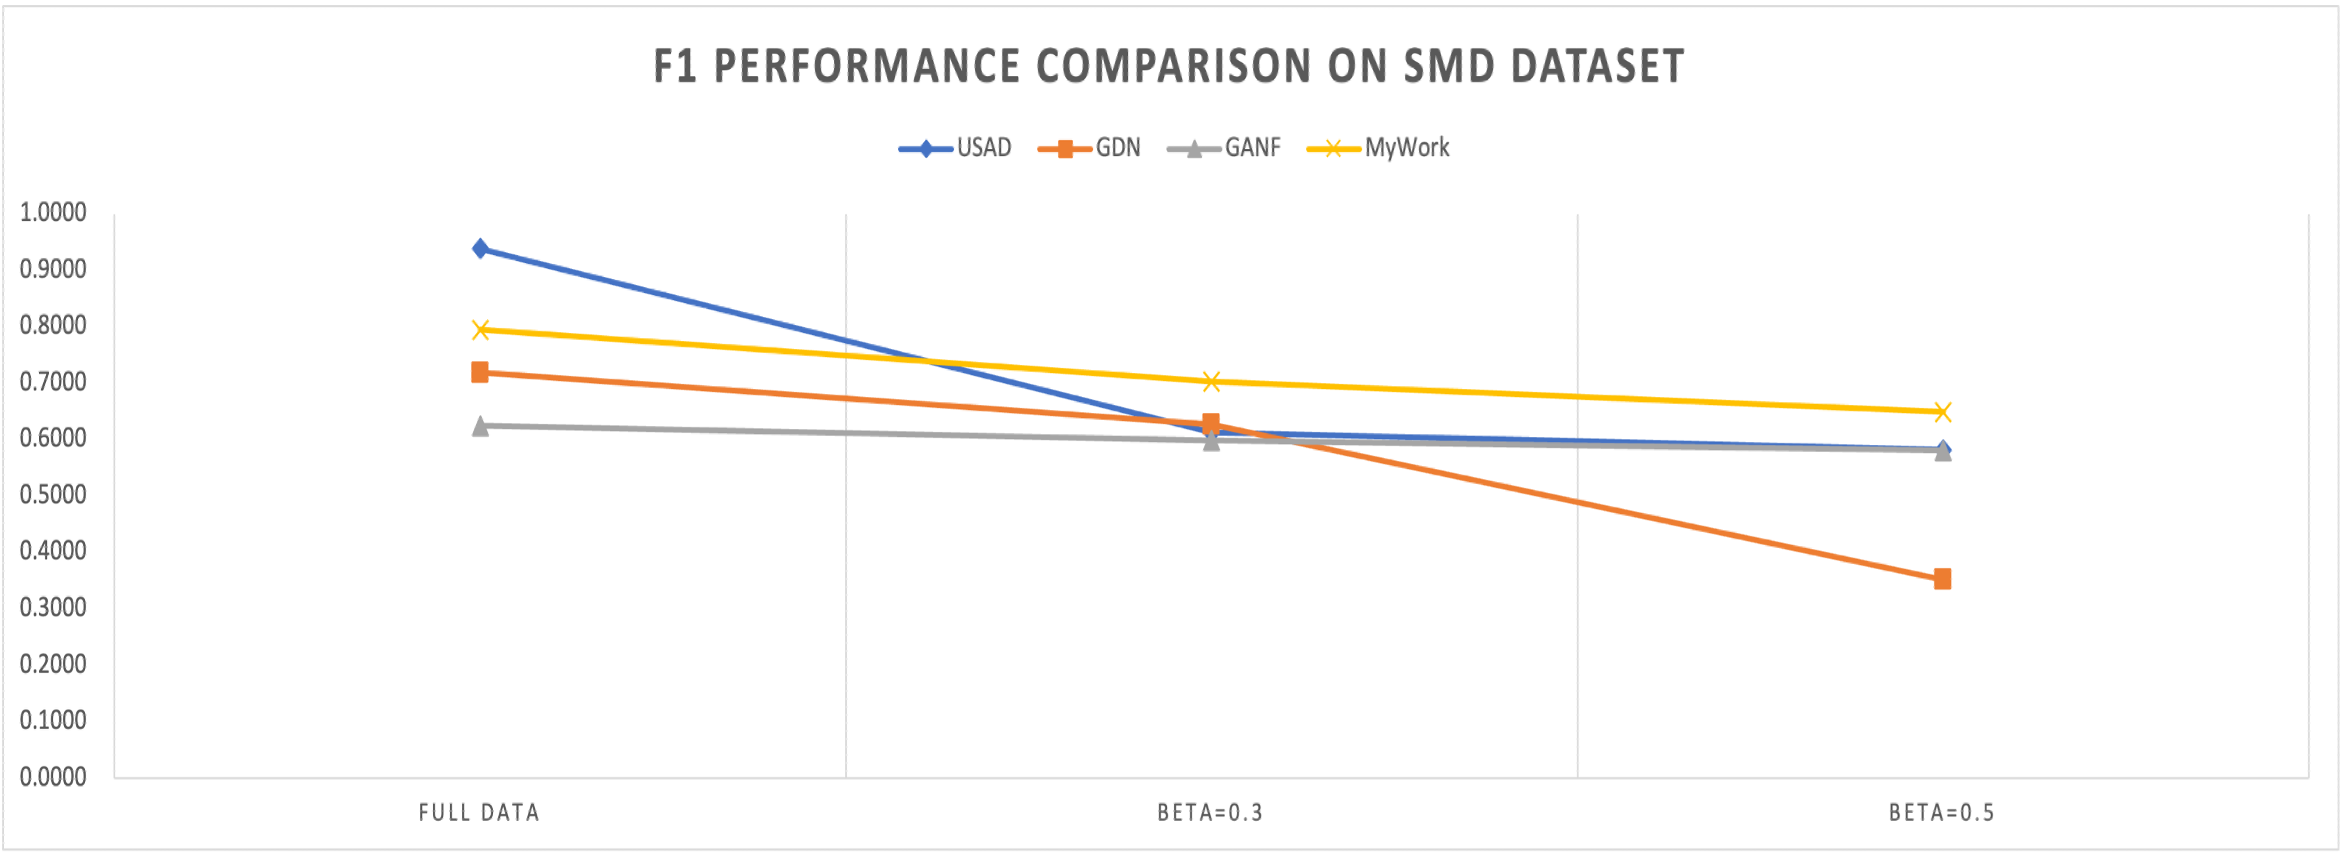
\includegraphics[width = 0.8\textwidth]{chapter4/smd-comapre.png}
  \caption{所有方法在SMD数据集上的性能比较}
  \end{figure}
图4-3展示了SMD 数据集中对比结果,其中横坐标代表缺失值场景,纵坐标代表F1综合性能分数。可以看到我们在完整数据集下的性能接近当前的SOTA方案,在30\%缺失值的情况下
对比SOTA方案提升约为17\%至12\%,在在50\%缺失值的情况下对比SOTA方案提升约为84\%至11\%。


常见的缺失值填充方法有填充默认值、均值、众数、KNN填充等。其中填充固定值选取某个固定值/默认值填充缺失值。其中对每一列的缺失值,填充当列的均值。填充均值得是对每一列的缺失值,
填充当列的中位数。填充众数指的是对每一列的缺失值,填充当列的众数。填充上下条的数据指的是对每一条数据的缺失值,填充其上下条数据的值。
由于传统多元时间序列异常检测模型只能在不包含缺失值的数据集上执行异常检测任务,因此在对比传统多元时间序列异常检测模型在包含缺失值的数据集上的性能表现时必须要
先对缺失值进行填充。需要注意的是,对于异常检测任务,我们只能使用检测时刻之前的历史数据进行填充而不能使用检测时刻之后的未来数据进行填充。在此条件的限制下,
我们为每个对比方法先验得在sklearn提供的经典数据填充方法(均值填充,中位数填充,常数填充,众数填充)中选择效果最好的填充方法,最终对比方法为 
USAD+Mean, GDN+Mean, GANF+Median。

如表4-4, 表4-5, 表4-6所示,我们测试了不同程度下删除数据后模型性能表现。通过实验结果我们可以看到,我们在SOTA模型的原场景下接近SOTA的性能,
同时在我们设计的新的场景下超过SOTA模型的表现,以此可以证明我们的模型在缺失值场景下具有较好的性能表现。
同时我们的模型在beta = 0 至 beta = 0.3 与 beta = 0.3 至 beta = 0.5 的场景变换中,性能下降最低,这证明了我们的模型在数据损失的情况下性能
下降最不明显,对数据缺失具有鲁棒性。

\begin{table}[htb]
  \caption{填充数据集后所有方法在SWAT数据集上的性能比较}
  %\label{comparison_results}
  \small
  \centering
  \setlength{\tabcolsep}{0.8mm}{
  \begin{tabular}{lccccccccc}\toprule
  Method & \multicolumn{3}{c}{SMD FULL DATA} & \multicolumn{3}{c}{SMD DROP 0.3 DATA} & \multicolumn{3}{c}{SMD DROP 0.5 DATA} \\ \cmidrule(r){2-4} \cmidrule(r){5-7} \cmidrule(r){8-10}
      & F1-Score & Precision & Recall & F1-Score & Precision & Recall & F1-Score & Precision & Recall\\ \midrule
      USAD+Mean & 0.7917 & 0.9851 & 0.6618 & 0.59172 & 0.44499 & 0.88284 & 0.3818 & 0.25788 & 0.735315 \\
      GDN+Mean & 0.8100 & 0.9935 & 0.6812 & 0.69393 & 0.857535 & 0.58275 & 0.5948 & 0.763455 & 0.487305 \\
      GANF+Median & 0.8065 & 0.9892 & 0.6808 & 0.31996 & 0.212625 & 0.64617 & 0.1379 & 0.073815 & 1 \\
      MMTSAD & 0.7522 & 0.9583 & 0.6191 & 0.6886 & 0.8106 & 0.5986 & 0.6869 & 0.784 & 0.6112 \\
%\bfseries MUSE-Net& \bfseries 2.89 & \bfseries 1.10 & \bfseries 2.74 & \bfseries 1.05 & \bfseries 15.47 & \bfseries 5.47 & \bfseries 14.45 & \bfseries 5.54 & \bfseries 17.19 \\
\bottomrule
\centering
\end{tabular}}
\end{table}

\begin{table}[htb]
  \caption{填充数据集后所有方法在WADI数据集上的性能比较}
  %\label{comparison_results}
  \small
  \centering
  \setlength{\tabcolsep}{0.8mm}{
  \begin{tabular}{lccccccccc}\toprule
  Method & \multicolumn{3}{c}{SMD FULL DATA} & \multicolumn{3}{c}{SMD DROP 0.3 DATA} & \multicolumn{3}{c}{SMD DROP 0.5 DATA} \\ \cmidrule(r){2-4} \cmidrule(r){5-7} \cmidrule(r){8-10}
      & F1-Score & Precision & Recall & F1-Score & Precision & Recall & F1-Score & Precision & Recall\\ \midrule
      USAD+Mean & 0.2328 & 0.9947 & 0.1318&  0.2243 & 0.267855 & 0.19299 & 0.1959&  0.19918 & 0.19278 \\
      GDN+Mean & 0.5700 & 0.9750 & 0.4019 & 0.1458 & 0.08421 & 0.543585 & 0.2067 & 0.11466 & 1 \\
      GANF+Mean & 0.3348 & 0.2040 & 0.9324 & 0.2345 & 0.14658 & 0.58632 & 0.1826&  0.175035&  0.19089 \\
      MMTSAD & 0.3897 & 0.2718 & 0.6883 & 0.2821 & 0.2102 & 0.4286  & 0.2179 & 0.2179 & 0.5844 \\
%\bfseries MUSE-Net& \bfseries 2.89 & \bfseries 1.10 & \bfseries 2.74 & \bfseries 1.05 & \bfseries 15.47 & \bfseries 5.47 & \bfseries 14.45 & \bfseries 5.54 & \bfseries 17.19 \\
\bottomrule
\centering
\end{tabular}}
\end{table}

\begin{table}[htb]
  \caption{填充数据集后所有方法在SMD数据集上的性能比较}
  %\label{comparison_results}
  \small
  \centering
  \setlength{\tabcolsep}{0.8mm}{
  \begin{tabular}{lccccccccc}\toprule
  Method & \multicolumn{3}{c}{SMD FULL DATA} & \multicolumn{3}{c}{SMD DROP 0.3 DATA} & \multicolumn{3}{c}{SMD DROP 0.5 DATA} \\ \cmidrule(r){2-4} \cmidrule(r){5-7} \cmidrule(r){8-10}
      & F1-Score & Precision & Recall & F1-Score & Precision & Recall & F1-Score & Precision & Recall\\ \midrule
      USAD+Mean & 0.9382 & 0.9314 & 0.9617 & 0.6435 & 0.494865 & 0.92001 & 0.6109 & 0.46116 & 0.904785 \\
      GDN+Mean & 0.7183 & 0.7079 & 0.7294 & 0.6577 & 0.625275 & 0.693735 & 0.3693 & 0.24822 & 0.721455 \\
      GANF+Median & 0.6241 & 0.5131 & 0.7963 & 0.6282 & 0.501795 & 0.84 & 0.6098 & 0.445935 & 0.964425 \\
      MMTSAD & 0.7949 & 0.9051 & 0.7086 & 0.7025 & 0.7367 & 0.6714& 0.6491 & 0.5881 & 0.7243 \\
%\bfseries MUSE-Net& \bfseries 2.89 & \bfseries 1.10 & \bfseries 2.74 & \bfseries 1.05 & \bfseries 15.47 & \bfseries 5.47 & \bfseries 14.45 & \bfseries 5.54 & \bfseries 17.19 \\
\bottomrule
\centering
\end{tabular}}
\end{table}

我们通过设置以下三种情况来验证模型各个模块的有效性,即:
\begin{enumerate}
  \item Full model: 不修改模型
  \item Drop MMAR: 删除时间位置编码模块以及掩码注意力表征模块
  \item Drop CNF-AD: 用一个简单的全连接层决策(正常/异常)结果
\end{enumerate}

如表所示,我们在缺失值为0.3的SWAT数据集和缺失值为0.5的SWAT数据集上进行了消融实验,实验结果表明删除时间位置编码模块以及掩码注意力表征模块后的模型(Drop MMAR)在两种场景下相比较完整的模型性能
分别下降了27\%和49\%;删除CNF-AD模块后的模型在两种场景下性能下降分别为(34\%和38\%)。

通过消融实验我们得到了以下结果:Drop MMAR 性能下降,证明了MMAR能够有效表征缺失值多元时间序列,Drop MMAR 性能下降率 与 数据确实率成正比,证明了MMAR对不同缺失值场景下具有鲁棒性, Drop CNF-AD 性能下降,证明了 CNF-AD能够有效识别异常。

\begin{table}[ht]
  \caption{消融实验性能比较}
  %\label{comparison_results}
  \small
  \centering
  \setlength{\tabcolsep}{0.8mm}{
  \begin{tabular}{lcccccc}\toprule
  Method & \multicolumn{3}{c}{SWAT DROP 0.3 DATA} & \multicolumn{3}{c}{SWAT DROP 0.5 DATA}  \\ \cmidrule(r){2-4} \cmidrule(r){5-7} 
      & F1-Score & Precision & Recall & F1-Score & Precision & Recall \\ \midrule
      full model & 0.6886 & 0.8106 & 0.5986  & 0.6869 & 0.784 & 0.6112 \\
      drop MMAR & 0.5734 (-27\%) & 0.6282 & 0.6036  & 0.3405(-49\%) & 0.2117  & 0.8706 \\ 
      drop CNF-AD & 0.4578(-34\%) & 0.3207 & 0.7996  & 0.4958 (-38\%)&  0.4933 &  0.6133\\       
%\bfseries MUSE-Net& \bfseries 2.89 & \bfseries 1.10 & \bfseries 2.74 & \bfseries 1.05 & \bfseries 15.47 & \bfseries 5.47 & \bfseries 14.45 & \bfseries 5.54 & \bfseries 17.19 \\
\bottomrule
\centering
\end{tabular}}
\end{table}

\section{本章小节}[Introduction]
本文针对工业场景中更加常见的含缺失值时间序列异常检测任务,提出一种基于注意力重新表征的时间序列异常检测算法。该算法首先将包含缺失值的时间序列数据通过时间位置编码对时间序列中不同时间戳关联性进行建模;然后通过掩码注意力表征模块学习不同时间戳之间数据的关联关系并表征为一个高维的嵌入式编码矩阵;最后引入条件标准化流对数据进行重建,以重建概率作为数据异常评分。最后本章做了两部分实验,其中第一部分为性能实验,对比MMTSAD与当前多元时间序列异常检测SOTA在三种缺失值场景下的性能表现;第二部分为消融实验,分析不同模块在完成异常检测任务过程的效果。